
\chapter{INTRODUÇÃO}

O desenvolvimento de tecnologias ligadas a telecomunicação tem alcançado novos limites levando em consideração o aumento da utilização de equipamentos de comunicação sem fio. Dessa forma, a demanda por eficiência em projetos relacionados tem demandado uma maior taxa de transferência visando um aproveitamento melhor do uso da tecnologia. Tendo isso em vista, a transmissão de bandas múltiplas concorrentes, transmissão de dois ou mais sinais ao mesmo tempo, vem sendo uma estratégia adotada para aumentar as taxas de transmissão de dados, reduzindo o custo e tendo uma maior eficiência espectral\cite{8070682}. Sob essa perspectiva, os amplificadores de potência (PA) desempenham um papel fundamental, pois são responsáveis por amplificar o sinal antes da antena de transmissão, permitindo sua propagação a longas distâncias.
Embora fundamentais, os amplificadores de potência constituem componentes críticos no sistema \cite{martins2011eficiencia}. Tais dispositivos demandam um alto consumo de energia e operam frequentemente com baixa eficiência, além de inserirem distorções no sinal quando fora de sua região de linearidade;fenômenos atrelados a fatores construtivos inerentes ao equipamento.

A preservação das características do sinal requer que o amplificador atue em sua região de linearidade, condição que, limita a eficiência energética do sistema. Como alternativa para otimizar o consumo, é recorrente a operação do PA próximo à sua região de saturação. Essa prática, embora vantajosa do ponto de vista energético, aumenta as não linearidades do dispositivo e degrada a informação transmitida. Para mitigar tais distorções, a técnica de pré-distorção digital(DPD) é amplamente adotada \cite{9427989}, pois permite compensar os efeitos inerentes do amplificador e garantir a linearidade do sistema como um todo.

A pré-distorção digital atua como um modelo posicionado antes do amplificador de potência na cadeia de transmissão, projetado para modelar o inverso da função característica do PA. Em termos operacionais, o DPD modela o sinal ao introduzir uma distorção, de modo que a resposta combinada do pré-distorcedor e do amplificador resulte em um sistema linear \cite{alvarado2019papr}. Este condicionamento é imprescindível para resguardar a máscara espectral do sinal, atenuando os produtos de intermodulação e as emissões fora de banda que causam interferência em canais adjacentes. Desse modo, o DPD não apenas garante o cumprimento dos rigorosos requisitos regulatórios de espectro, mas também permite que o PA opere em regiões de maior eficiência, garantindo um balanço ideal entre linearidade e consumo energético.

Conforme a Figura \ref{dpd_pa}, a linearização do sistema pode ser observada por meio do comportamento de três estágios: a inserção prévia de distorção pelo DPD, a distorção natural imposta pelo PA e a saída combinada, que idealmente resulta em uma resposta linear. Operando como a função inversa do amplificador, o DPD viabiliza o cumprimento dos rigorosos requisitos de qualidade espectral e viabiliza operações mais eficientes.
Apesar dos ganhos promovidos pela pré-distorção, a manutenção da eficiência energética do transmissor em patamares aceitáveis exige o uso de abordagens adicionais. Nesse contexto, destacam-se as técnicas dedicadas à redução da Relação Potência de Pico a Potência Média (PAPR, do inglês \textit{Peak-to-Average Power Ratio}), visto que elevados picos de sinal forçam o amplificador a operar em regiões menos eficientes para evitar o ceifamento da onda.

\begin{figure}[H]
	\centering
	\caption{LINEARIDADE DPD E PA}
	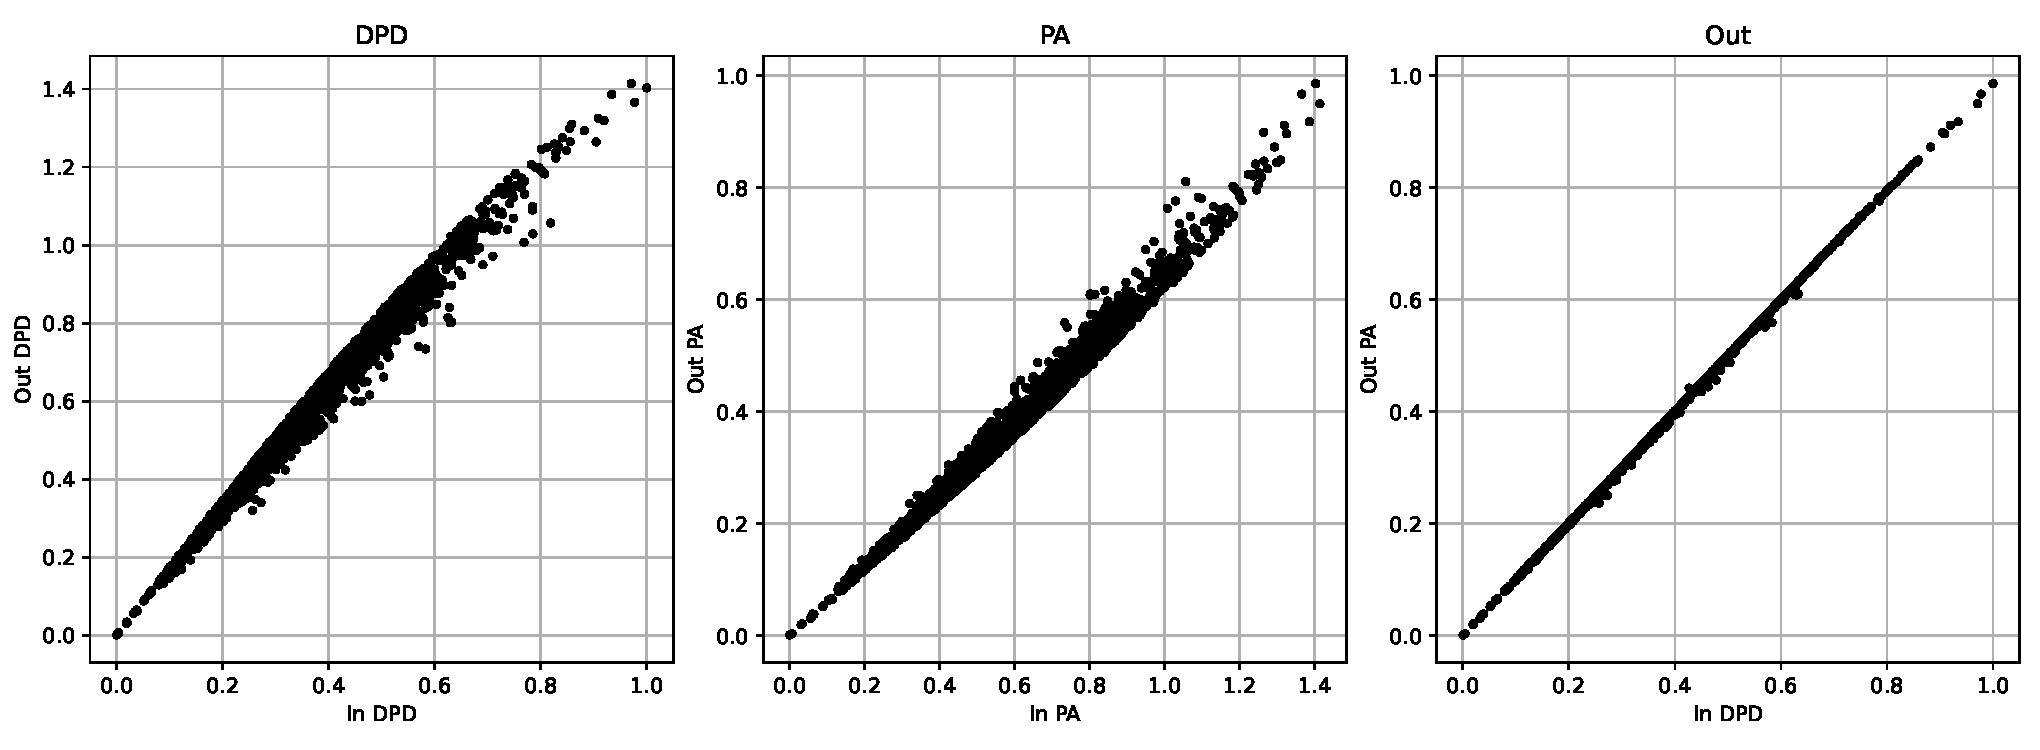
\includegraphics[width=0.75\linewidth]{fig/Linearidade_PA_DPD.pdf}
	\caption*{FONTE: AUTOR}
	\label{dpd_pa}
\end{figure}

Para atenuar os elevados níveis de PAPR, uma estratégia recorrente é o ceifamento do sinal antes de ser enviado ao DPD. O princípio elementar dessa técnica é o \textit{hard clipping}, onde a tensão do sinal é truncada ao atingir um limiar específico. Ao operar com uma única banda, a limitação é simplificada, visto que a amplitude corresponde à envoltória isolada do sinal. Em contrapartida, em arranjos de múltiplas bandas, como a coexistência de um sinal Wi-Fi (2,4 GHz) e LTE (3,5 GHz) abordada neste trabalho, a envoltória composta deriva da sobreposição espectral, inviabilizando a análise individual das portadoras. Diante disso, a literatura consolida duas vertentes principais para a aplicação do ceifamento: a abordagem da soma e a abordagem da divisão. Deve-se ressaltar, contudo, que essa truncagem abrupta induz o espalhamento espectral, gerando componentes de frequência  fora da banda de interesse. Tal espalhamento pode infringir normas regulatórias, provocando interferência de canal adjacente e comprometendo a integridade das comunicações de sinais que se encontram em frequências próximas.


A Figura \ref{SISTEMA PROPOSTO COM FILTROS.} exemplifica a implementação proposta, dado que a saturação do sinal ocasiona um espalhamento espectral, espalhando a frequência além dos limites impostos, a solução é a implementação de um filtro FIR, \textit{Finite Impulse Response}, localizado antes do pré-distorsor para conter o sinal dentro de uma faixa especificada. Esta estratégia foi validada na literatura por \cite{oliveira2025fir_complete}, apresentando bons resultados na contenção das emissões fora de banda. Contudo, a presente aplicação identifica uma oportunidade de aprimoramento focada na redução da ordem do filtro implementado.

\begin{figure}[H]
	\centering
	\caption{SISTEMA PROPOSTO COM FILTROS.}
	\input{tik.tex}
	\caption*{FONTE: AUTOR}
	\label{SISTEMA PROPOSTO COM FILTROS.}
\end{figure}

\section{Objetivos}
O presente trabalho tem como objetivo principal a redução  do tamanho do filtro sem comprometer a funcionalidade utilizando técnicas de síntese dos filtros com base nas restrições das normas e em otimização não linear.
\subsection{Objetivos Específicos}
Para os objetivos específicos, tem-se:
\begin{itemize}
	\item Redução do número de coeficientes na implementação do filtro;
	\item Não alteração dos resultados alcançados com a implementação do filtro, de forma a manter os valores já alcançados;
	\item Validar a implementação dos resultados no domínio do tempo.
\end{itemize}


